\documentclass{beamer}
\usepackage[british,spanish]{babel}
\usepackage[utf8]{inputenc}
\usepackage{hyperref}
\usepackage{multirow}



\usepackage{listings}

\usepackage{adjustbox}
\usepackage{lstcustom}

\usepackage{color}
\definecolor{light-gray}{gray}{0.80}
\definecolor{lstbackgroundshellcolor}{named}{light-gray}

\usepackage{tikz}
\newcommand*\circled[1]{\tikz[baseline=(char.base)]{
            \node[shape=circle,draw,inner sep=2pt] (char) {#1};}}

\usepackage[normalem]{ulem}

%\usepackage[acronym,xindy,toc]{glossaries}

\usepackage[acronym,xindy,toc]{glossaries}
\makeglossaries
%\usepackage[xindy]{imakeidx}
%\makeindex

\newcommand{\comment}[2]{#2}

\graphicspath{ {./images/} }

\title[Cloud Computing with Amazon Web Services]{Scaling with Amazon Web Services}
%\subtitle[short subtitle]{long subtitle}
\author[C. Cuenca, F. Quintana]{Carmelo Cuenca-Hernández and Francisca Quintana-Domínguez}
%\institute{Escuela Universitaria de Informática}
%\date[04/2013]{Abril - 2013}
\date{}
\titlegraphic{
\includegraphics[width=0.5 \textwidth]{images/awslogo.eps}}

\newcommand{\outputcommand}[1]{\color{darkgreen}{#1}}

\pgfdeclareimage[width=2.0\baselineskip]{ulpgc-logo}{images/logosimbolo_secundario_version_vertical}
\setbeamertemplate{footline}{\raisebox{-2ex}{\pgfuseimage{ulpgc-logo}}
  \usebeamerfont{date in head/foot}\insertshortdate{}\hfill
  \usebeamertemplate{navigation symbols}\hfill
  \insertframenumber{}/\inserttotalframenumber}
\setbeamertemplate{sidebar right}{}


\usetheme{Antibes}
%\usetheme{Berlin}

%\usetheme{Warsaw}
%\usecolortheme{albatross}

\begin{document}

\begin{frame}
	\titlepage
\end{frame}


\section*{Outline}
\begin{frame}
  \frametitle{Outline}
  %\tableofcontents%[part=1,pausesections]
  %\tableofcontents[currentsection,currentsubsection, sectionstyle=show] 
  \tableofcontents[currentsection,sectionstyle=show,hideothersubsections]
\end{frame}


\selectlanguage{british}

%%%%%%%%%%%%%%%%%%%%%%%%%%%%%%%%%%%%%%%%%%%%%%%%%%%%%%%%%%%%%%%%%%%%%%%%%%%%%%
%\newacronym{<label>}{<abbrv>}{<full>}
%\glsreset{<label>}
%\glsresetall
%\acrlong{<label>}
%\acrfull{<label>}
%\acrshort{<label>}
\newacronym{ami}{AMI}{Amazon Machine Image}
\newacronym{aws}{AWS}{Amazon Web Services}
\newacronym{ebs}{EBS}{Elastic Block Storage}
\newacronym{ec2}{EC2}{Amazon Elastic Compute Cloud}
\newacronym{ecu}{ECU}{Elastic Compute Unit}
\newacronym{elb}{ELB}{Elastic Load Balancing}
\newacronym{rds}{RDS}{Relational Database Service}
\newacronym{s3}{S3}{Simple Storage Service}
\newacronym{sqs}{SQS}{Amazon Simple Queue Service}
%%%%%%%%%%%%%%%%%%%%%%%%%%%%%%%%%%%%%%%%%%%%%%%%%%%%%%%%%%%%%%%%%%%%%%%%%%%%%%
\section{Scaling with Amazon Web Services}
\begin{frame}[fragile]
\frametitle{Scaling with Amazon Web Services}
\begin{itemize}
 \item All you need \dots
 \begin{itemize}
   \item A desktop or laptop (with Internet access, of course)
   \item A credit card (for setting up an AWS account)
   \item A phone (to complete the registration process)
 \end{itemize}
\end{itemize}
\begin{center}
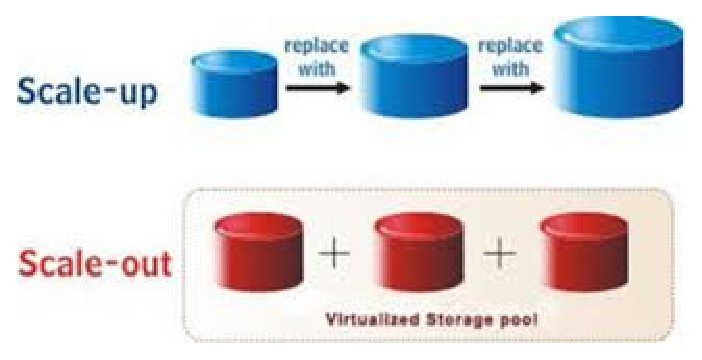
\includegraphics[scale=0.6]{scale.eps}
\end{center}
\end{frame}
%%%%%%%%%%%%%%%%%%%%%%%%%%%%%%%%%%%%%%%%%%%%%%%%%%%%%%%%%%%%%%%%%%%%%%%%%%%%%%
\begin{frame}[fragile]
\frametitle{Choosing an Architecture}
\begin{itemize}
 \item We have a standard, three-tiered application, consisting of a database, an application server, and a web server
\end{itemize}
\begin{center}
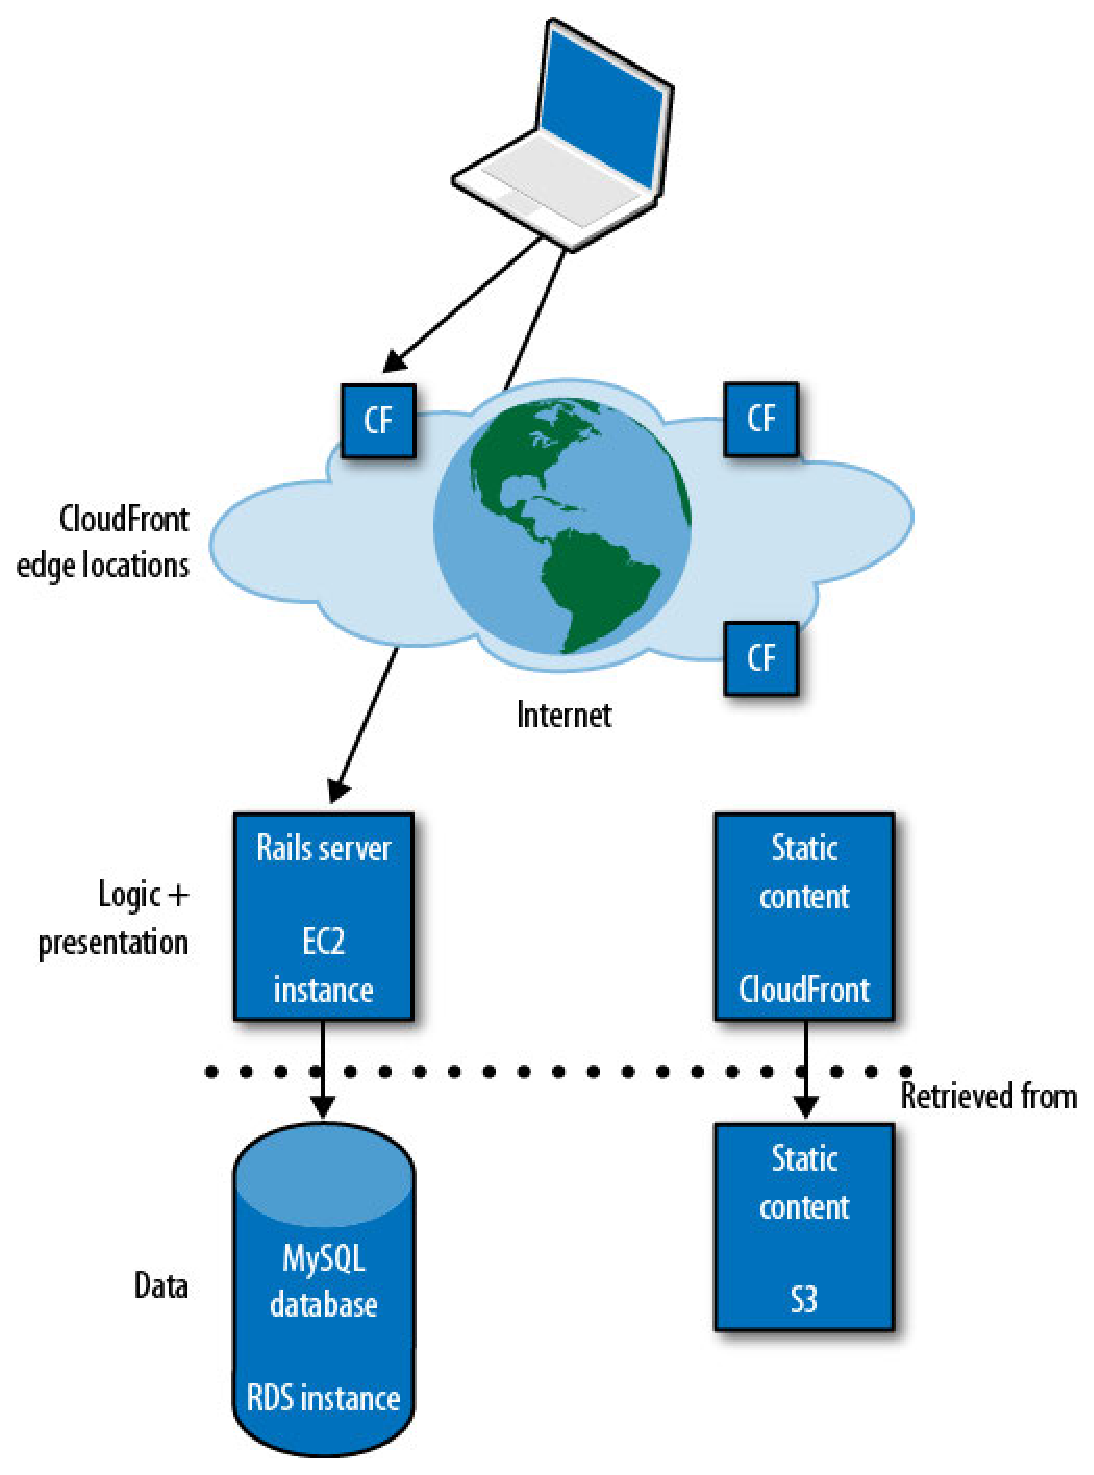
\includegraphics[scale=0.20]{Programming_Amazon_EC2-013.eps}
\end{center}
\end{frame}
%%%%%%%%%%%%%%%%%%%%%%%%%%%%%%%%%%%%%%%%%%%%%%%%%%%%%%%%%%%%%%%%%%%%%%%%%%%%%%
\section{RDS Database}
\begin{frame}[fragile, allowframebreaks]
\frametitle{RDS Database}
\begin{itemize}
 \item \acrfull{rds} is a web service that makes it easy to set up, operate, and scale a relational database in the cloud
 \item It provides cost-efficient and resizable capacity while managing time-consuming database administration tasks, freeing you up to focus on your applications and business
 \item \acrshort{rds} gives you access to the capabilities of a familiar \texttt{MySQL}, \texttt{Oracle}, \texttt{Microsoft SQL Server}, or \texttt{PostgreSQL} database engine
\end{itemize}
\begin{center}
      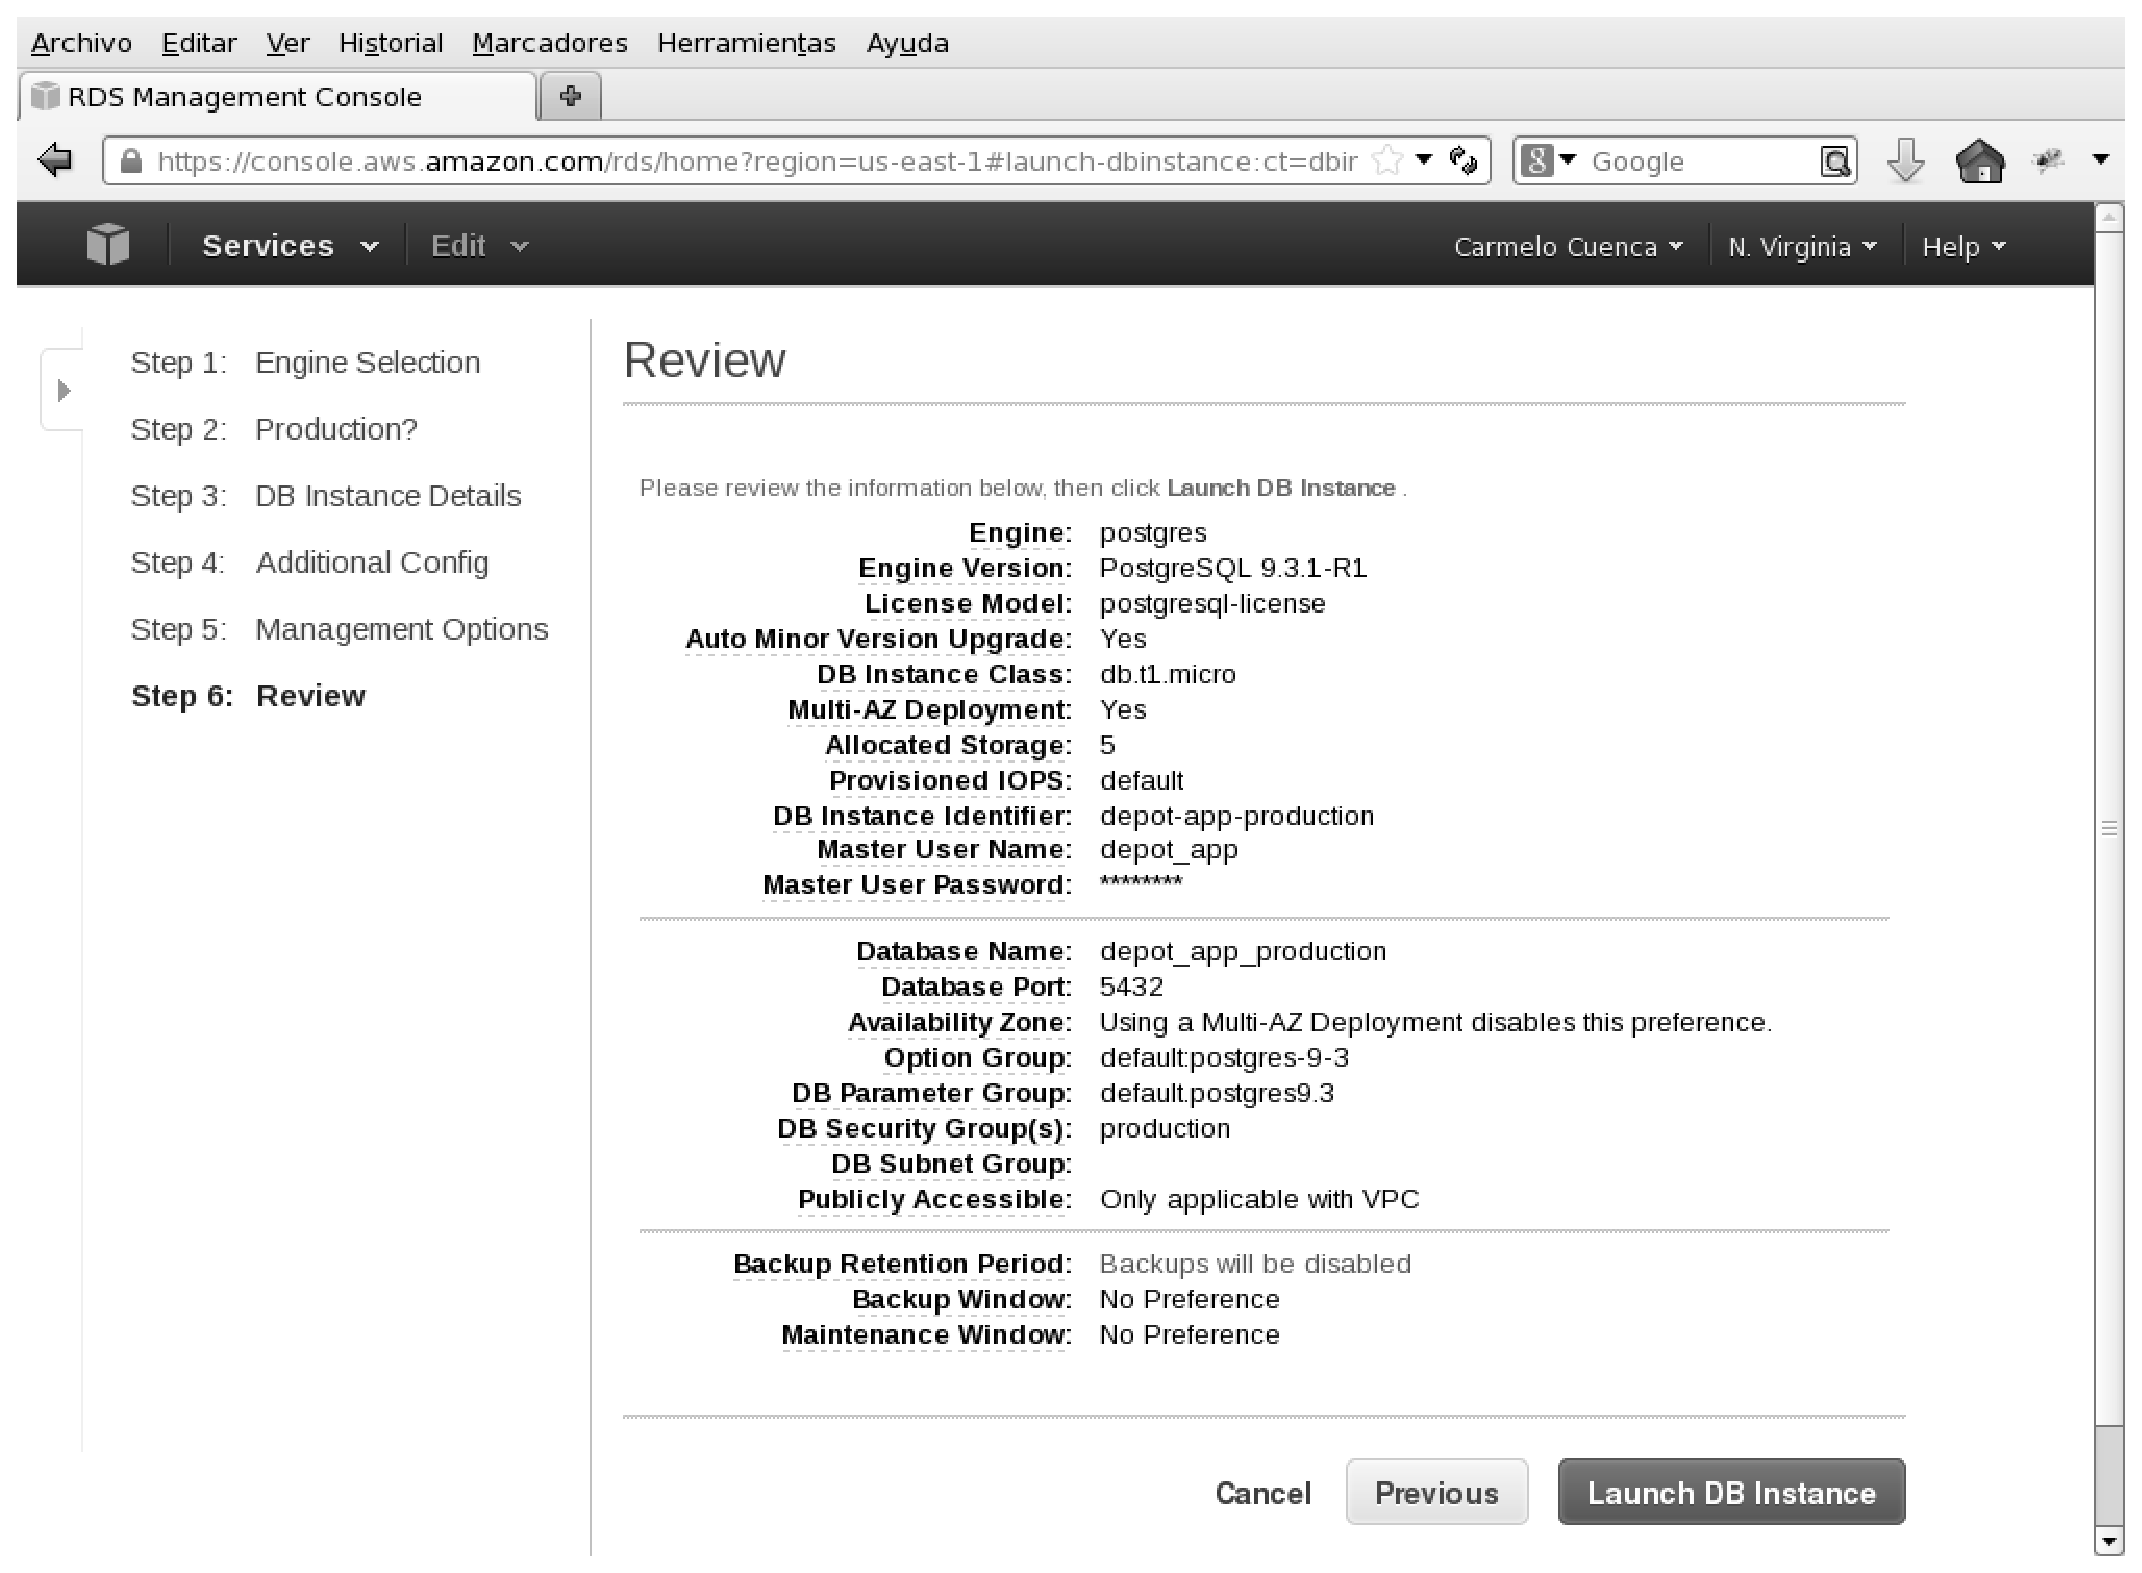
\includegraphics[scale=0.25]{rds.eps}
\end{center}
\end{frame}
%%%%%%%%%%%%%%%%%%%%%%%%%%%%%%%%%%%%%%%%%%%%%%%%%%%%%%%%%%%%%%%%%%%%%%%%%%%%%%
\begin{frame}[fragile, allowframebreaks]
\frametitle{DB Security Groups}
It is a good idea to create a DB security group. You can create the DB security group through the AWS Console and add the authorizations.
An authorization is a security group from an EC2 account that allows you to
share RDS instances easily across multiple accounts. Alternatively, you can specify a
CIDR/IP, much like we did for the EC2 security groups. For now, we will allow everyone
access to the DB instances in this group. Later, we’ll restrict that access again. You can
add a DB instance to multiple DB security groups, giving you the necessary flexibility
in case you work with multiple EC2 accounts

\begin{center}
      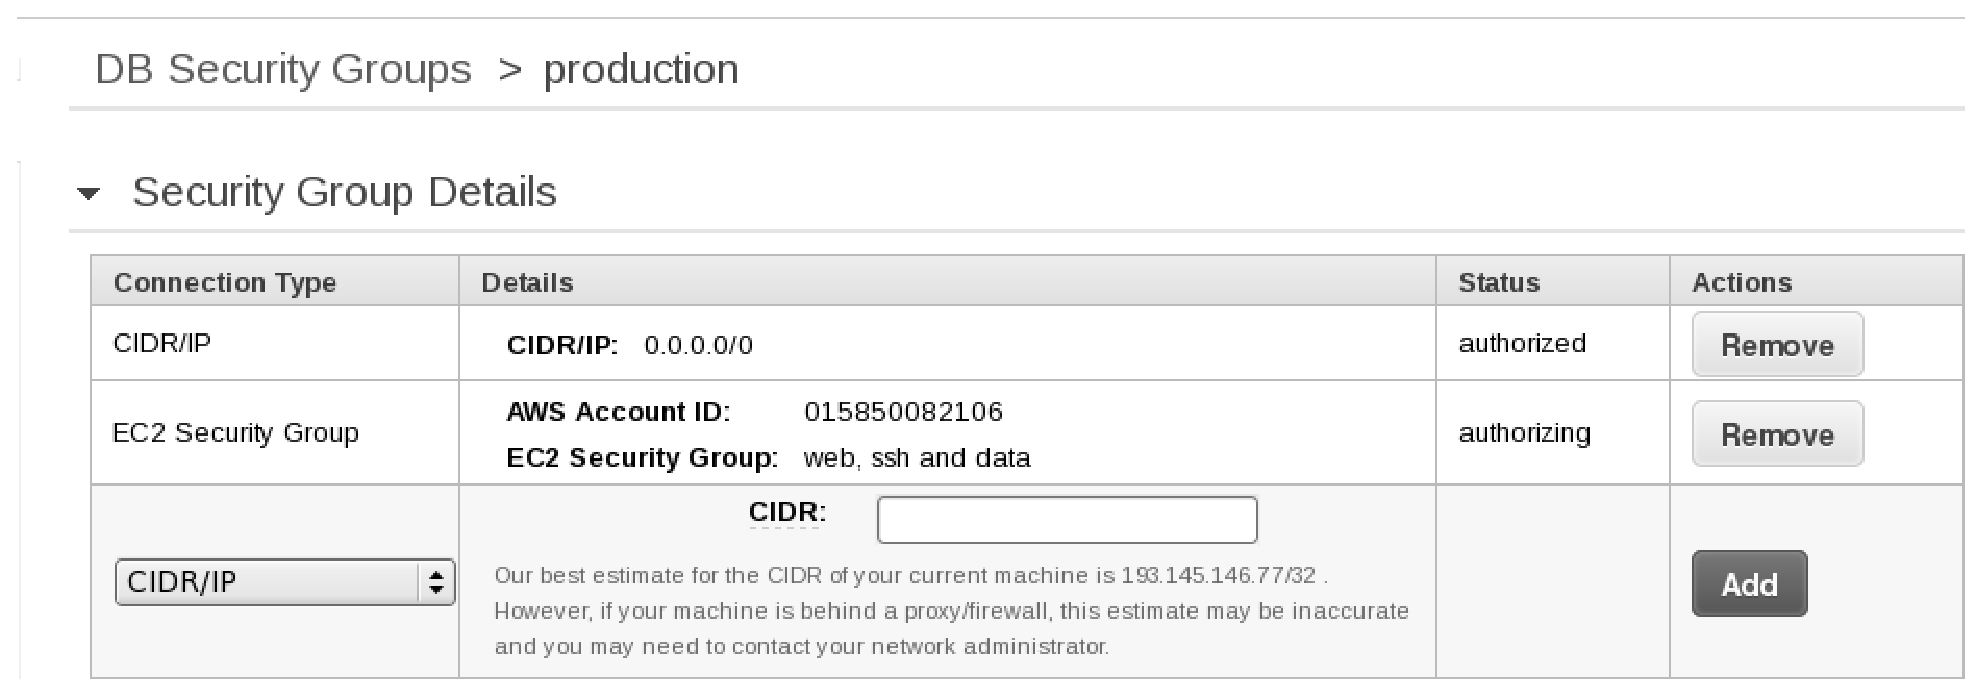
\includegraphics[scale=0.25]{securitydb.eps}
\end{center}
\end{frame}
%%%%%%%%%%%%%%%%%%%%%%%%%%%%%%%%%%%%%%%%%%%%%%%%%%%%%%%%%%%%%%%%%%%%%%%%%%%%%%
\begin{frame}[fragile, allowframebreaks]
\frametitle{Creating a RDS Instance}
\begin{itemize}
 \item Engine Selection (PostgreSQL)
 \item Production? Do you plan to use this database for production purposes?
    \begin{itemize}
      \item Multi-AZ Deployment for high availability (99.95\% monthly up time SLA). Provisioned IOPS Storage for fast, consistent performance
      \item Instance is intended for use outside of production or under the \alert{RDS Free Usage Tier}
    \end{itemize}
 \item DB Instance Details (Choose ``depot-app-production'' like \texttt{DB Instance Identifier} (hint: \texttt{DB Instance Identifier} must contain only letters, digits, or hyphens) and \texttt{Master Password} must be at least 8 characteres)
  \item Additional Config (Choose ``depot\_app\_production'' like \texttt{Database Name:} and ``production'' like \texttt{DB Security Group(s):})
  \item Management Options (Choose ``No'' for \texttt{Enabled Automatic Backups:}) 
  \item Review \& Laun DB Instance
  \end{itemize}
\end{frame}
%%%%%%%%%%%%%%%%%%%%%%%%%%%%%%%%%%%%%%%%%%%%%%%%%%%%%%%%%%%%%%%%%%%%%%%%%%%%%%%%%%%%%%%%%%%%%%%%%%%%%%%%%%%%%%%%%%%%%%%%%%%%%%%%%%%%%%%%%%
\begin{frame}[fragile, allowframebreaks]
\frametitle{Test a \acrshort{rds} Instance}
\begin{itemize}
 \item Test with a PostgreSQL client a \acrshort{rds} instance
 \lstset{language=shell, breaklines=true, escapechar=!}
  \begin{lstlisting}[escapechar=!]
  $ psql -W -h depot-app-production.ccoguny6ikux.us-east-1.rds.amazonaws.com  depot_app_production depot_app
  !\outputcommand{Contraseña para usuario depot\_app:\\
psql (9.3.2, servidor 9.3.1)\\
\dots}!
 \end{lstlisting}
 \end{itemize}
\end{frame}
%%%%%%%%%%%%%%%%%%%%%%%%%%%%%%%%%%%%%%%%%%%%%%%%%%%%%%%%%%%%%%%%%%%%%%%%%%%%%%%%%%%%%%%%%%%%%%%%%%%%%%%%%%%%%%%%%%%%%%%%%%%%%%%%%%%%%%%%%%
\begin{frame}[fragile, allowframebreaks]
\frametitle{Cloud PostgreSQL Database in Production Environments}
\begin{itemize}
\item Start and login in the \acrshort{ec2} instance

\lstset{language=shell, escapechar=!}
\begin{lstlisting}[escapechar=!]
$ ssh -i your_key_file.pem root@ec2-nnn-nnn-nn-nnn.compute-1.amazonaws.com
# su - depot_app
\end{lstlisting}

\item Edit \texttt{config/database.yml} file (configuration database file) in order to run the application with \texttt{PostgreSQL} \acrshort{rds}

\lstset{language=Ruby, style=eclipse, numbers=left}
\begin{lstlisting}[escapechar=!]
!\vdots!
production:
  adapter: postgresql
  encoding: unicode
  database: depot_app_production
  pool: 5
#!\circled{1}!
  host: depot-app-production.ccoguny6ikux.us-east-1.rds.amazonaws.com
  port: 5432
  username: depot_app
  password: 12345678
!\vdots!
\end{lstlisting}

\item Stop the PostgreSQL daemon

\lstset{language=shell, escapechar=!}
\begin{lstlisting}[escapechar=!]
# /etc/init.d/postgresql-9.3 stop
# chkconfig postgresql-9.3 off
# chkconfig --list postgresql-9.3
\end{lstlisting}

\item Migrate \texttt{depot\_app\_production} tables and  seed the data

\lstset{language=shell, style=eclipse}
\begin{lstlisting}[numbers=none, escapechar=!]
$ rake db:migrate RAILS_ENV=production
$ rake db:seed RAILS_ENV=production
\end{lstlisting}

\item Restart unicorn server
\lstset{language=shell, escapechar=!}
\begin{lstlisting}[escapechar=!]
# /etc/init.d/unicorn_depot_app restart
\end{lstlisting}

\item Curl your application and \dots 

\begin{lstlisting}[escapechar=!]
$ curl http://my.public.dns.amazonaws.com:5000
\end{lstlisting} 

 \end{itemize}
\end{frame}
%%%%%%%%%%%%%%%%%%%%%%%%%%%%%%%%%%%%%%%%%%%%%%%%%%%%%%%%%%%%%%%%%%%%%%%%%%%%%%%%%%%%%%%%%%%%%%%%%%%%%%%%%%%%%%%%%%%%%%%%%%%%%%%%%%%%%%%%%%
\begin{frame}[fragile, allowframebreaks]
\frametitle{Testing a Web Application}
\begin{itemize}
\item Tail user the Apachelog files  as \texttt{root}  in \acrshort{ec2} in order to check Apache Server
\lstset{language=shell}
\begin{lstlisting}[escapechar=!]
# tail -f /var/log/httpd/depot_app*
\end{lstlisting}
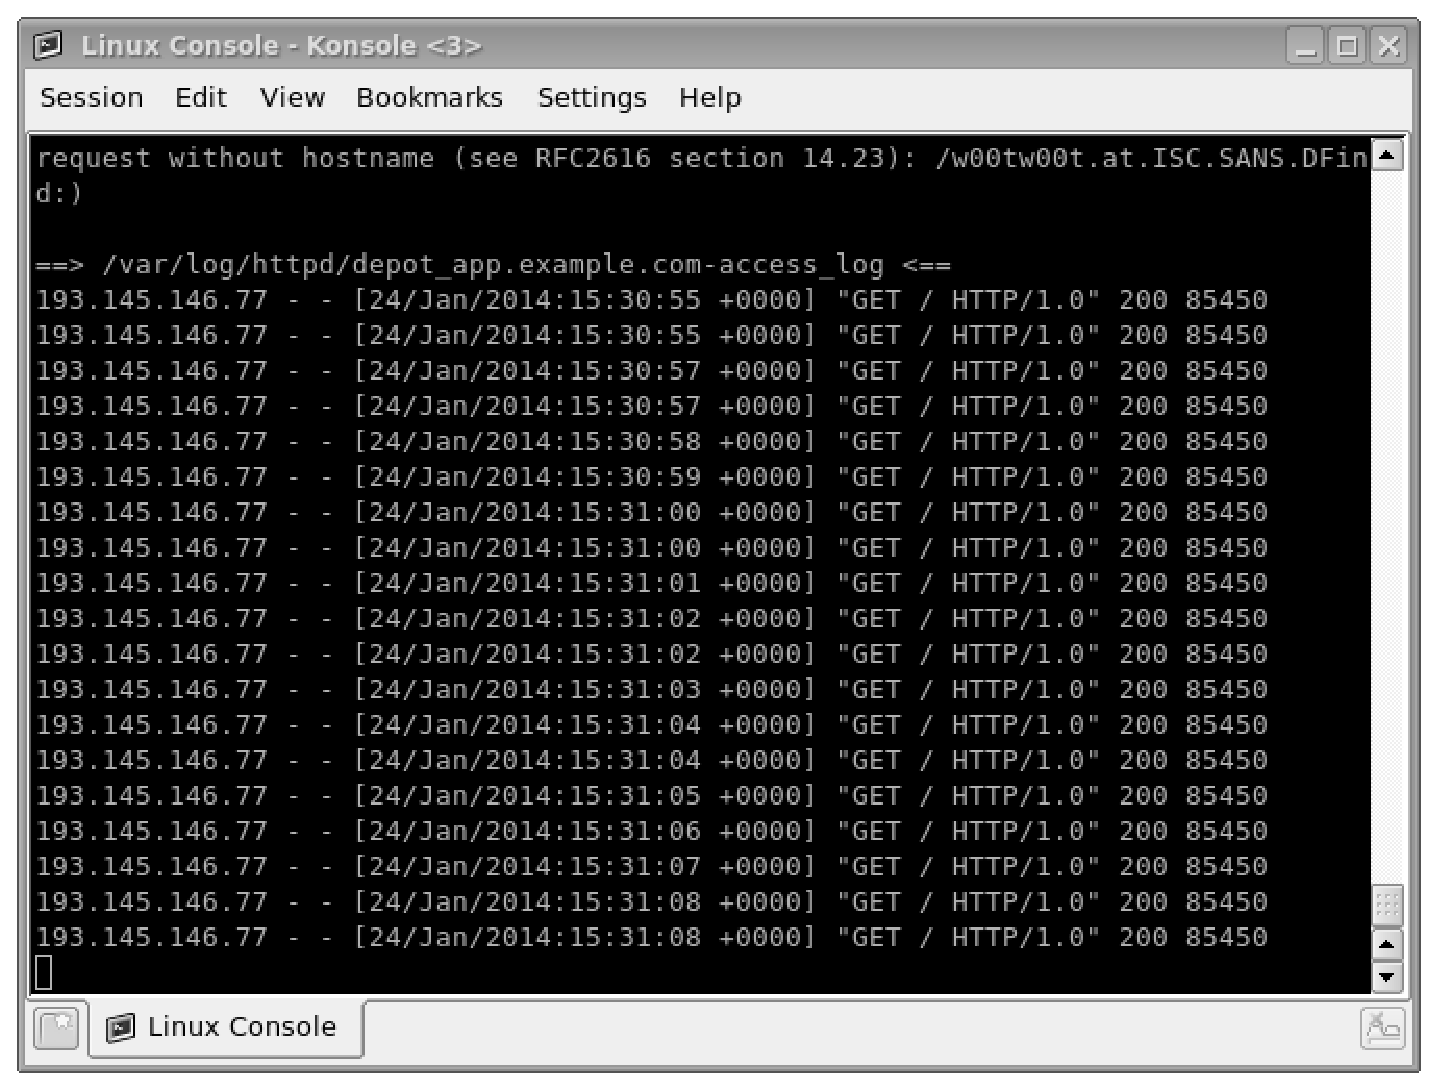
\includegraphics[scale=0.25]{logapache.eps}

\item Tail the Unicorn ( )log files as \texttt{depot\_app} in \acrshort{ec2} in order to check Unicorn Server
\lstset{language=shell}
\begin{lstlisting}[escapechar=!]
$ tail -f log/production.log log/unicorn.std*
\end{lstlisting}
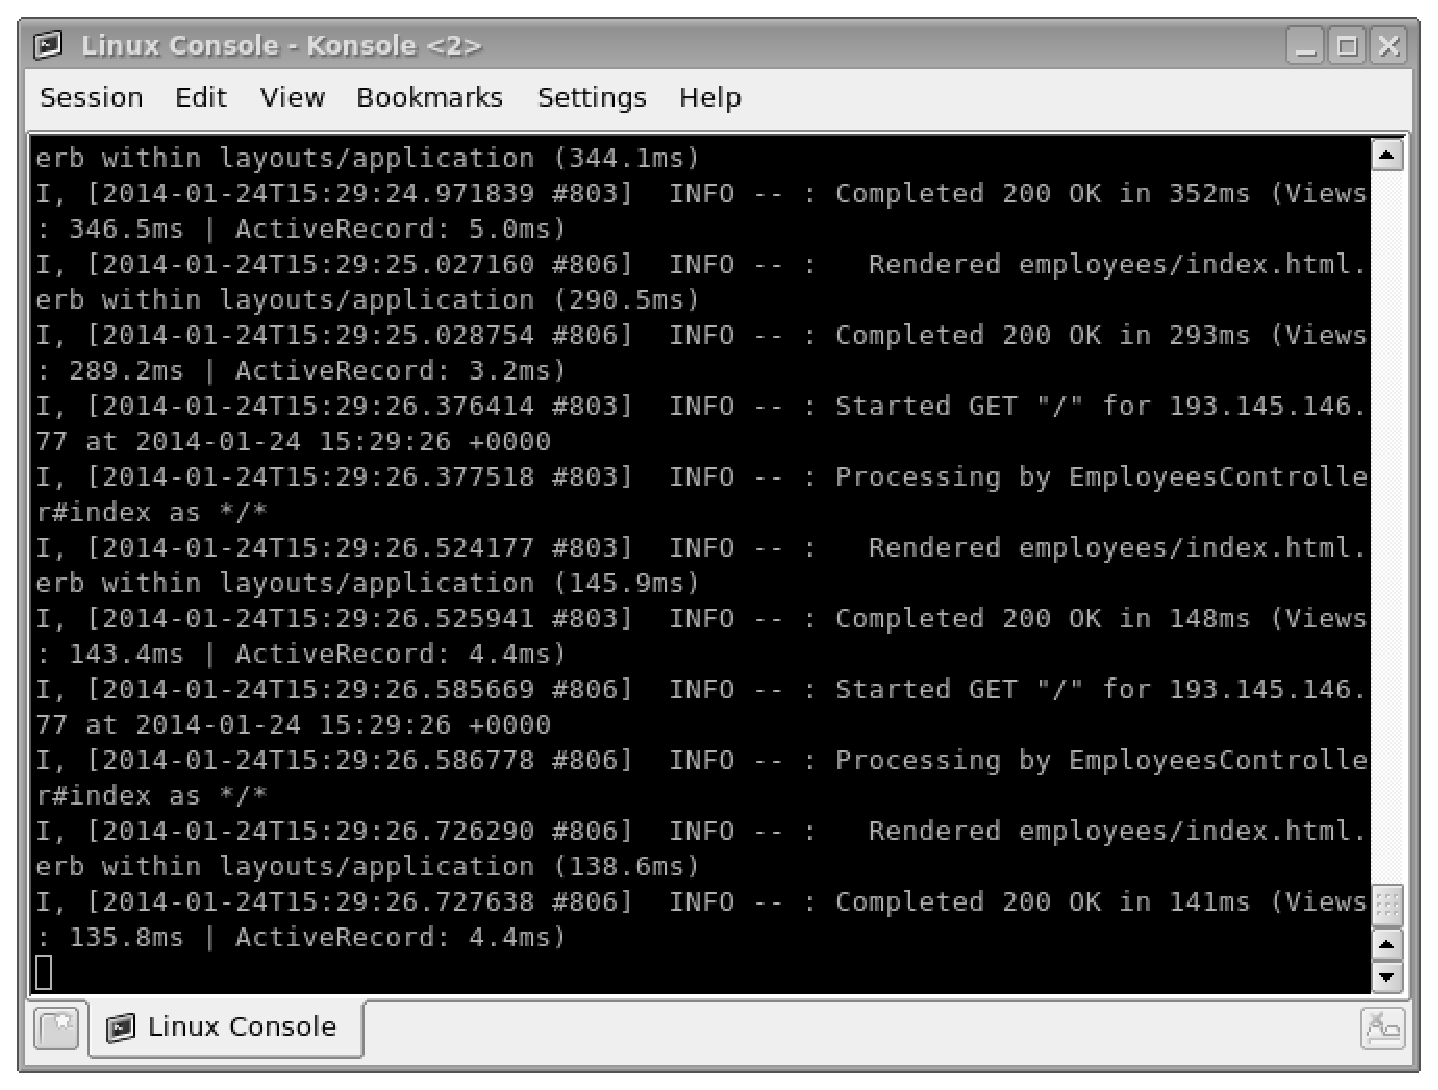
\includegraphics[scale=0.25]{lograils.eps}

\item Run Apache Bench \texttt{ab} in order to stress the Web Site

\lstset{language=shell}
\begin{lstlisting}[escapechar=!]
$ ab -n 60 -c 2  http://depot_app.com/
\end{lstlisting}


\lstset{language=shell}
\begin{lstlisting}[escapechar=!]
This is ApacheBench, Version 2.0.40-dev <$Revision: 1.146 $> apache-2.0
Copyright 1996 Adam Twiss, Zeus Technology Ltd, http://www.zeustech.net/
Copyright 2006 The Apache Software Foundation, http://www.apache.org/

Benchmarking depot_app.com (be patient).....done


Server Software:
Server Hostname:        depot_app.com
Server Port:            80

Document Path:          /
Document Length:        85450 bytes

Concurrency Level:      2
Time taken for tests:   43.910998 seconds
Complete requests:      60
Failed requests:        0
Write errors:           0
Total transferred:      5177820 bytes
HTML transferred:       5127000 bytes
Requests per second:    1.37 [#/sec] (mean)
Time per request:       1463.700 [ms] (mean)
Time per request:       731.850 [ms] (mean, across all concurrent requests)
Transfer rate:          115.14 [Kbytes/sec] received

Connection Times (ms)
              min  mean[+/-sd] median   max
Connect:      124  141  14.2    149     167
Processing:  1019 1301 174.2   1272    1931
Waiting:      266  357  76.1    346     625
Total:       1143 1443 183.2   1418    2082

Percentage of the requests served within a certain time (ms)
  50%   1418
  66%   1492
  75%   1562
  80%   1602
  90%   1679
  95%   1741
  98%   1851
  99%   2082
 100%   2082 (longest request)

\end{lstlisting}


\end{itemize}

\end{frame}
%%%%%%%%%%%%%%%%%%%%%%%%%%%%%%%%%%%%%%%%%%%%%%%%%%%%%%%%%%%%%%%%%%%%%%%%%%%%%%

%%%%%%%%%%%%%%%%%%%%%%%%%%%%%%%%%%%%%%%%%%%%%%%%%%%%%%%%%%%%%%%%%%%%%%%%%%%%%%
\section{S3/CloudFront}
%%%%%%%%%%%%%%%%%%%%%%%%%%%%%%%%%%%%%%%%%%%%%%%%%%%%%%%%%%%%%%%%%%%%%%%%%%%%%%
%%%%%%%%%%%%%%%%%%%%%%%%%%%%%%%%%%%%%%%%%%%%%%%%%%%%%%%%%%%%%%%%%%%%%%%%%%%%%%
\section{Amazon Machine Image (AMI)}
\begin{frame}[fragile, allowframebreaks]
\frametitle{Amazon Machine Image (AMI)}
\begin{enumerate}
\item You can customize the instance that you launch from a public \acrshort{ami} and then save that configuration as a custom \acrshort{ami} for your own use
\item Instances that you launch from your \acrshort{ami} use all the customizations that you've made
\end{enumerate}

\end{frame}
%%%%%%%%%%%%%%%%%%%%%%%%%%%%%%%%%%%%%%%%%%%%%%%%%%%%%%%%%%%%%%%%%%%%%%%%%%%%%%
%%%%%%%%%%%%%%%%%%%%%%%%%%%%%%%%%%%%%%%%%%%%%%%%%%%%%%%%%%%%%%%%%%%%%%%%%%%%%%
\begin{frame}[fragile, allowframebreaks]
\frametitle{Creating Your Own \acrshort{ami}}
\begin{enumerate}
\item In order to distinguish between \acrshort{ec2} machines change the application layout (as user \texttt{depot\_app} )

\lstset{language=html, style=eclipse}
\begin{lstlisting}[escapechar=!]
# ~/public_html/depot_app/app/views/layouts/application.html.erb
!\vdots!
  <div id="main">
    <%= yield %>
    <%= Socket.ip_address_list.to_s %> # !\circled{1}!
  </div>
</div>
\end{lstlisting}

\item Create an \acrshort{ami} of our \acrshort{ec2} instance and launch a new clone of our \acrshort{ec2} machine
\begin{center}
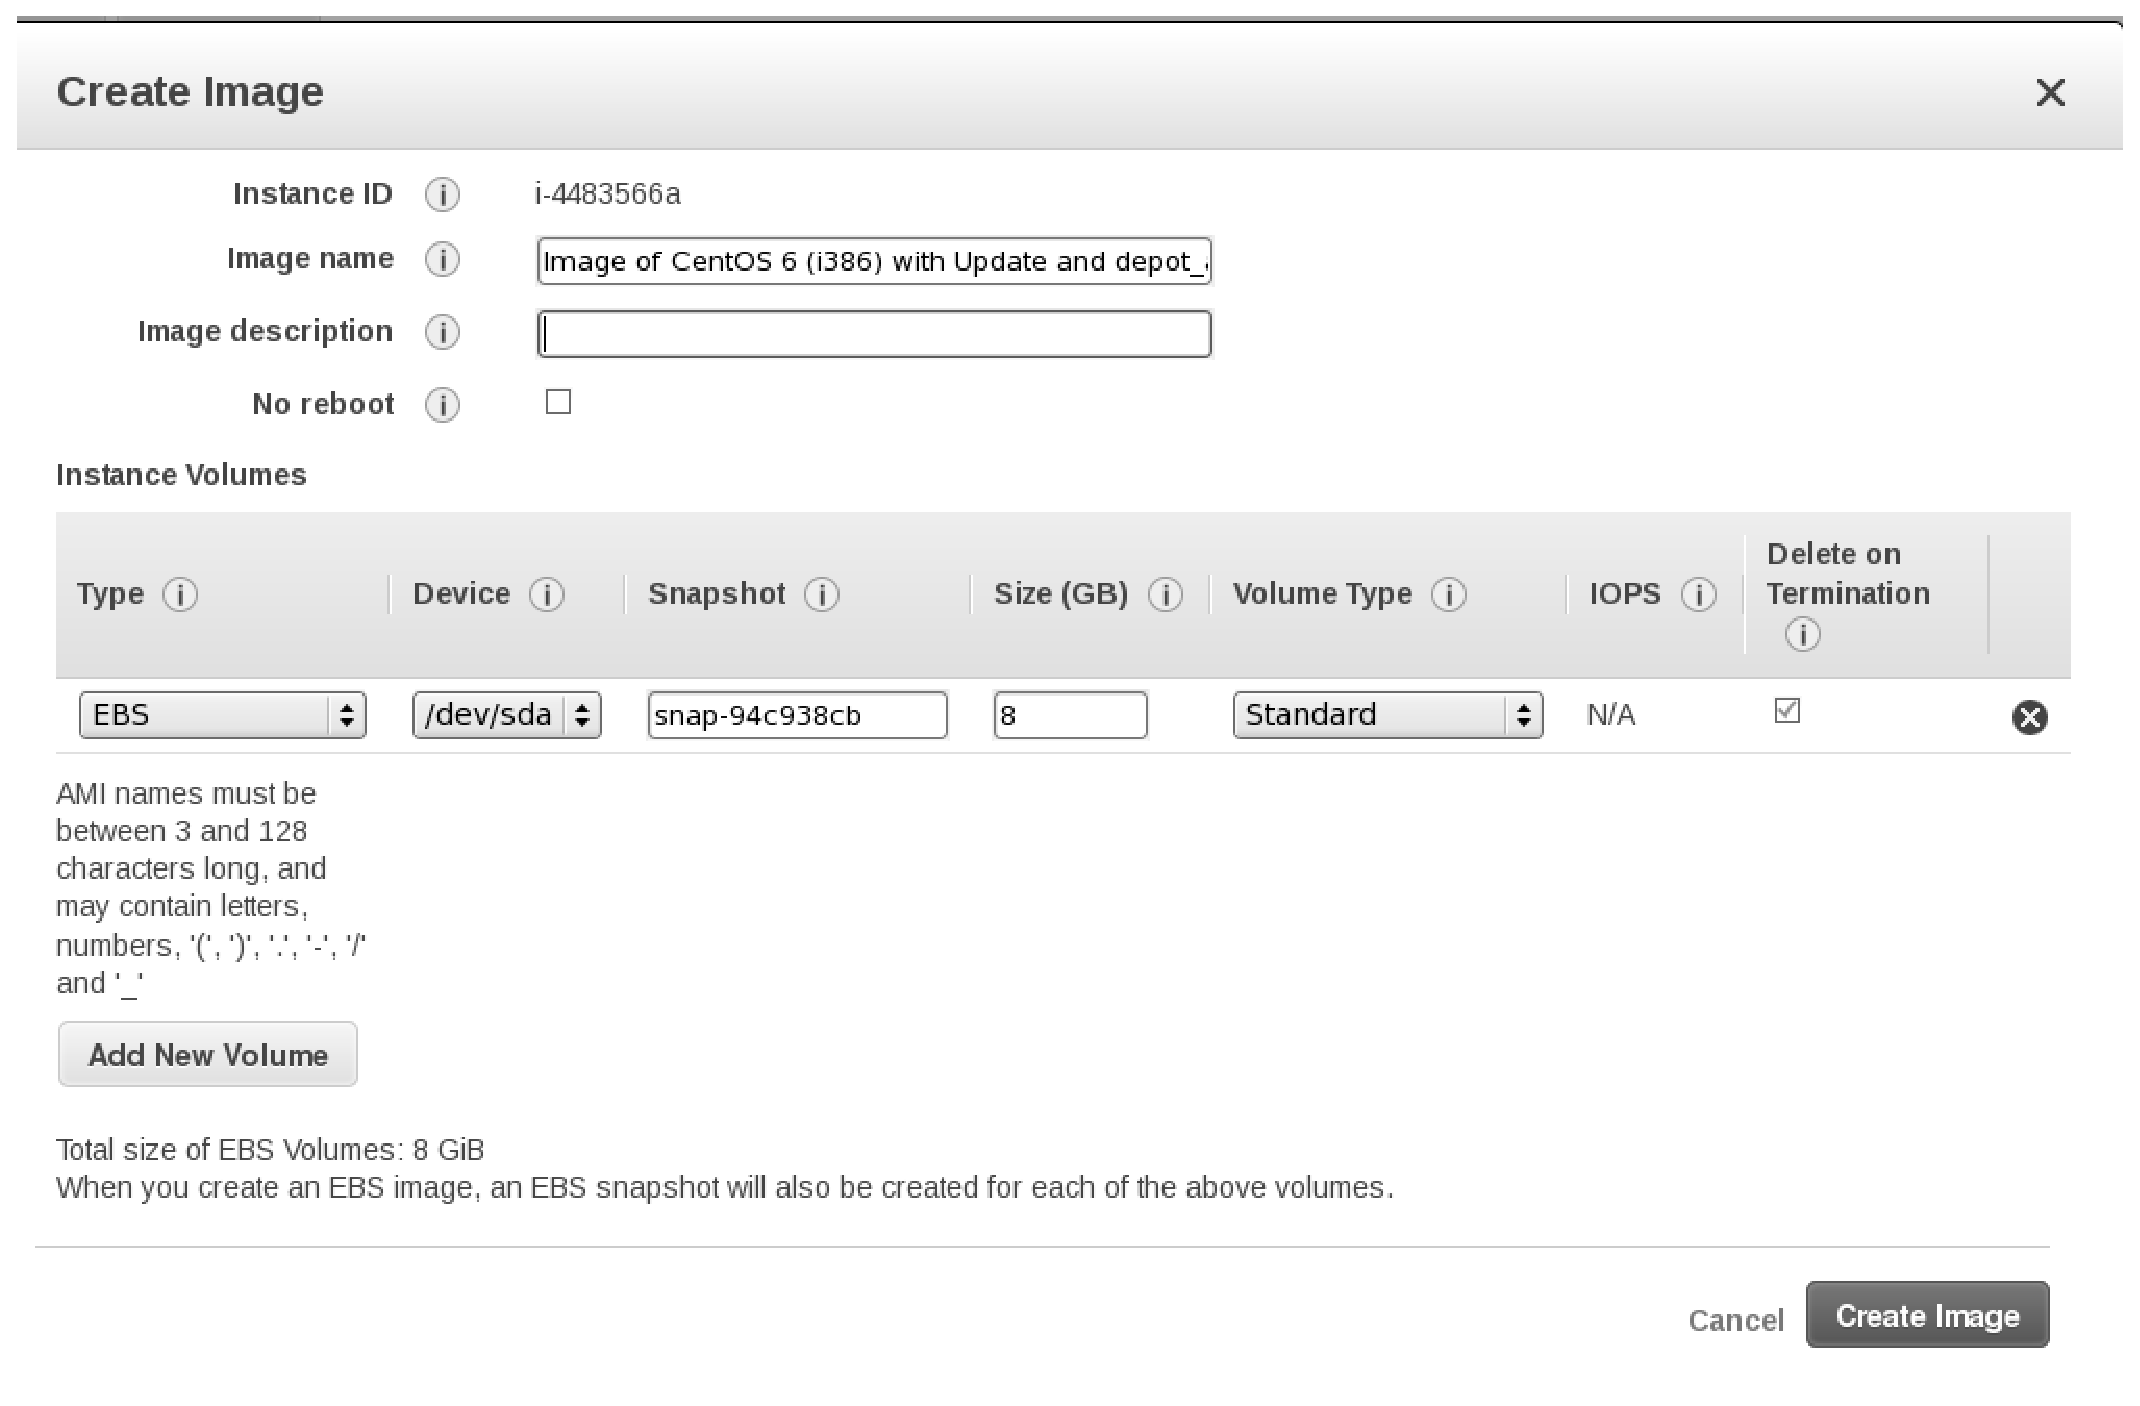
\includegraphics[scale=0.25]{createimage.eps}
\end{center}
\item Curl both IPs in order to test both \acrshort{ec2} instances
\end{enumerate}

\end{frame}
%%%%%%%%%%%%%%%%%%%%%%%%%%%%%%%%%%%%%%%%%%%%%%%%%%%%%%%%%%%%%%%%%%%%%%%%%%%%%%
%%%%%%%%%%%%%%%%%%%%%%%%%%%%%%%%%%%%%%%%%%%%%%%%%%%%%%%%%%%%%%%%%%%%%%%%%%%%%%
\section{Elastic Load Balancing}
%%%%%%%%%%%%%%%%%%%%%%%%%%%%%%%%%%%%%%%%%%%%%%%%%%%%%%%%%%%%%%%%%%%%%%%%%%%%%%
\begin{frame}[fragile, allowframebreaks]
\frametitle{Elastic Load Balancing}
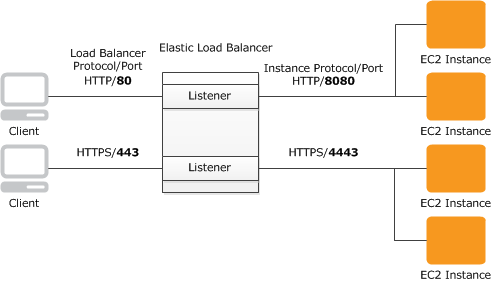
\includegraphics[width=0.75 \textwidth]{elb-listeners.png}
\begin{itemize}
\item Load balancing is ``a technique to distribute workload evenly across
two or more computers, network links, CPUs, hard drives, or other resources, in order
to get optimal resource utilization, maximize throughput, minimize response time, and
avoid overload.'' (Wikipedia)
\item  \acrfull{elb} checks the health of the
instances and will not route traffic to unhealthy instances
\item \acrshort{elb} is not a dedicated program or a hardware device; it is a load-balancing service. As
a service, it can automatically scale its capacity depending on incoming traffic. As a
result, an \acrshort{elb} is not referenced by an IP address, but by a fully qualified domain name
\end{itemize}
\end{frame}
%%%%%%%%%%%%%%%%%%%%%%%%%%%%%%%%%%%%%%%%%%%%%%%%%%%%%%%%%%%%%%%%%%%%%%%%%%%%%%
\begin{frame}[fragile, allowframebreaks]
\frametitle{Creating a ELB}
\begin{center}
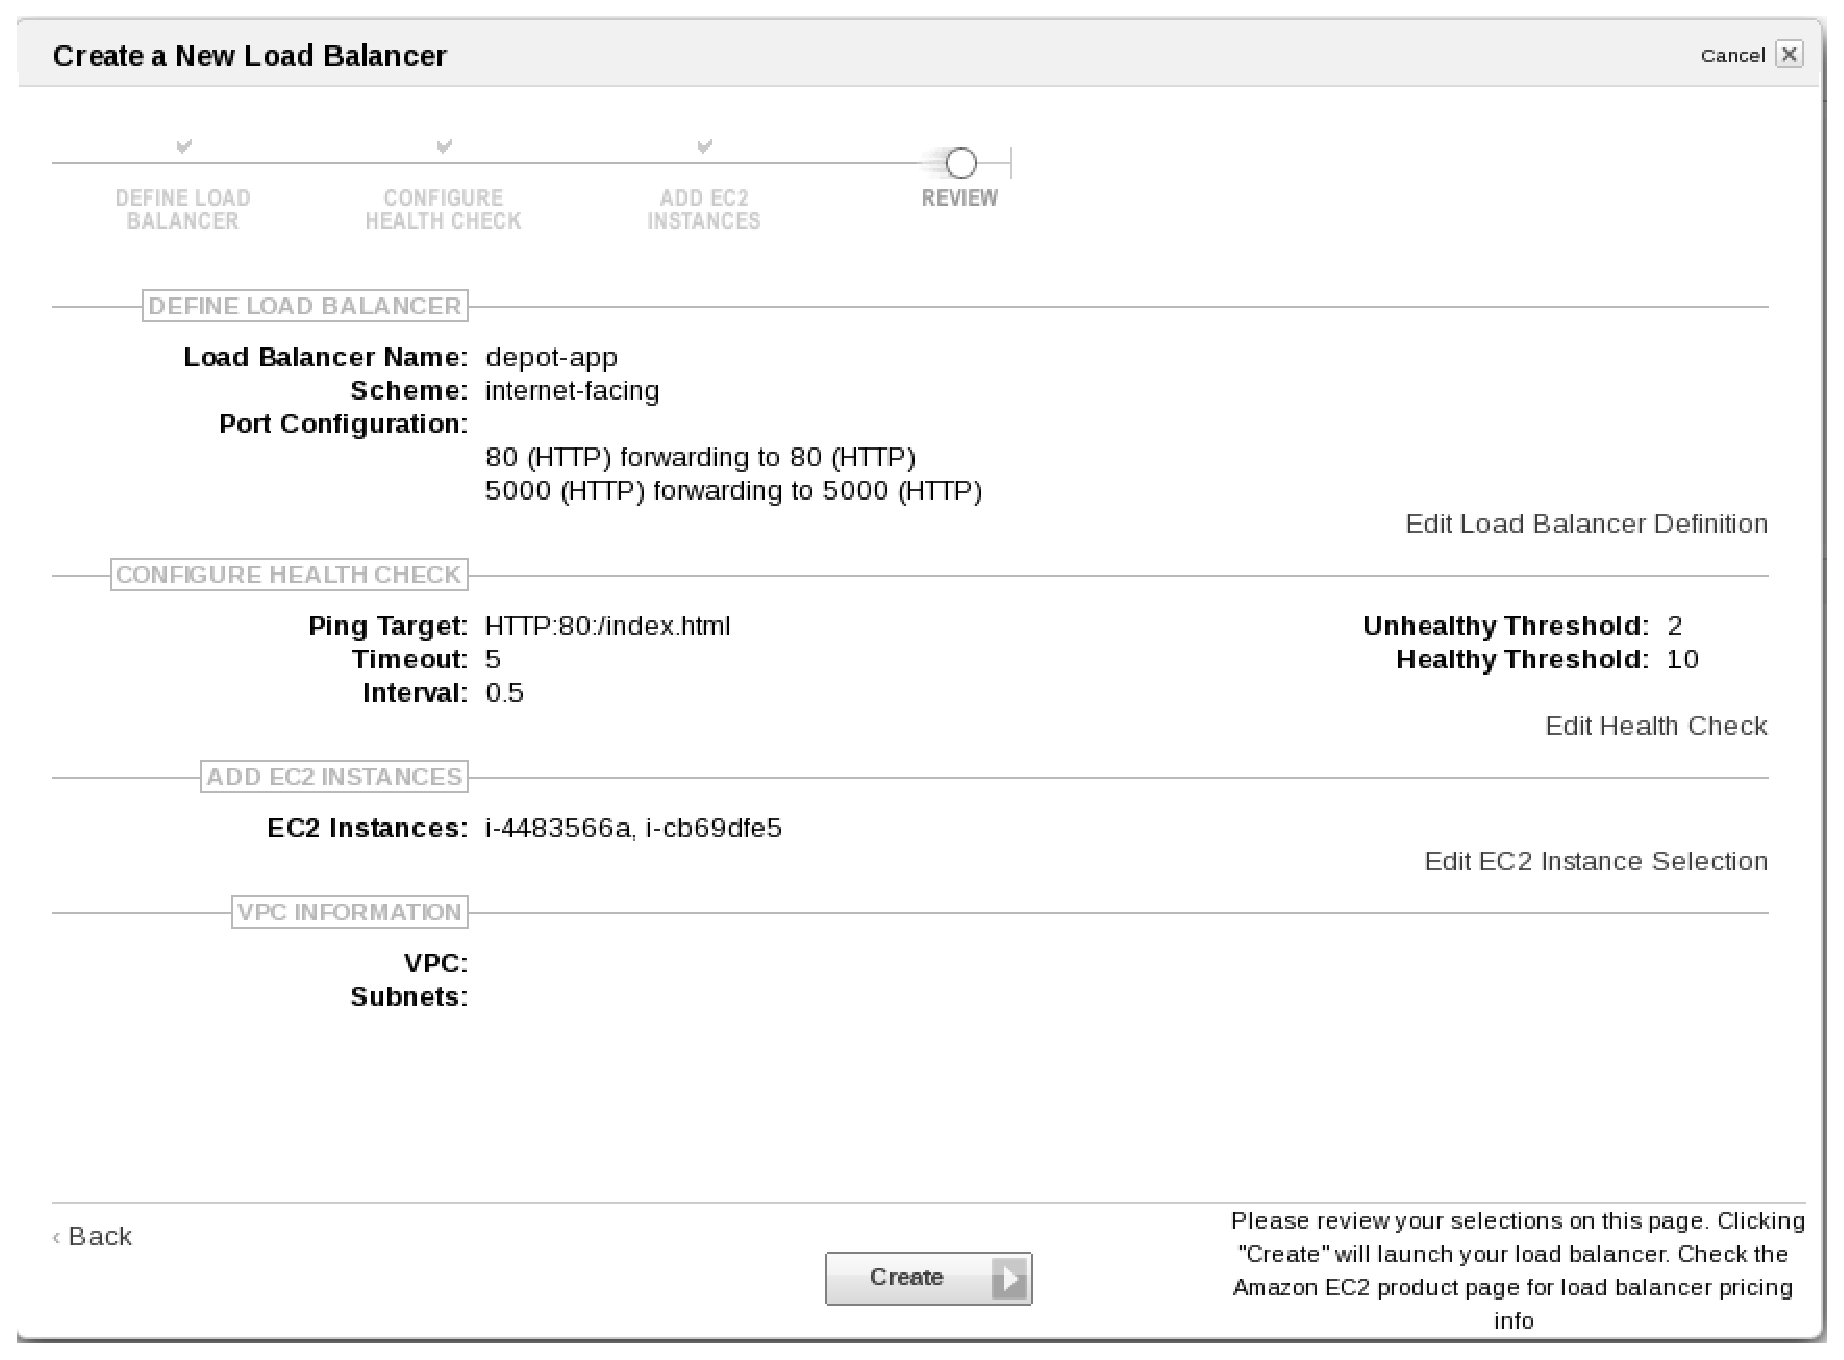
\includegraphics[scale=0.2]{readytocreate.eps}
\framebreak
\end{center}
\begin{enumerate}	
\item Define Load Balancer
\begin{center}
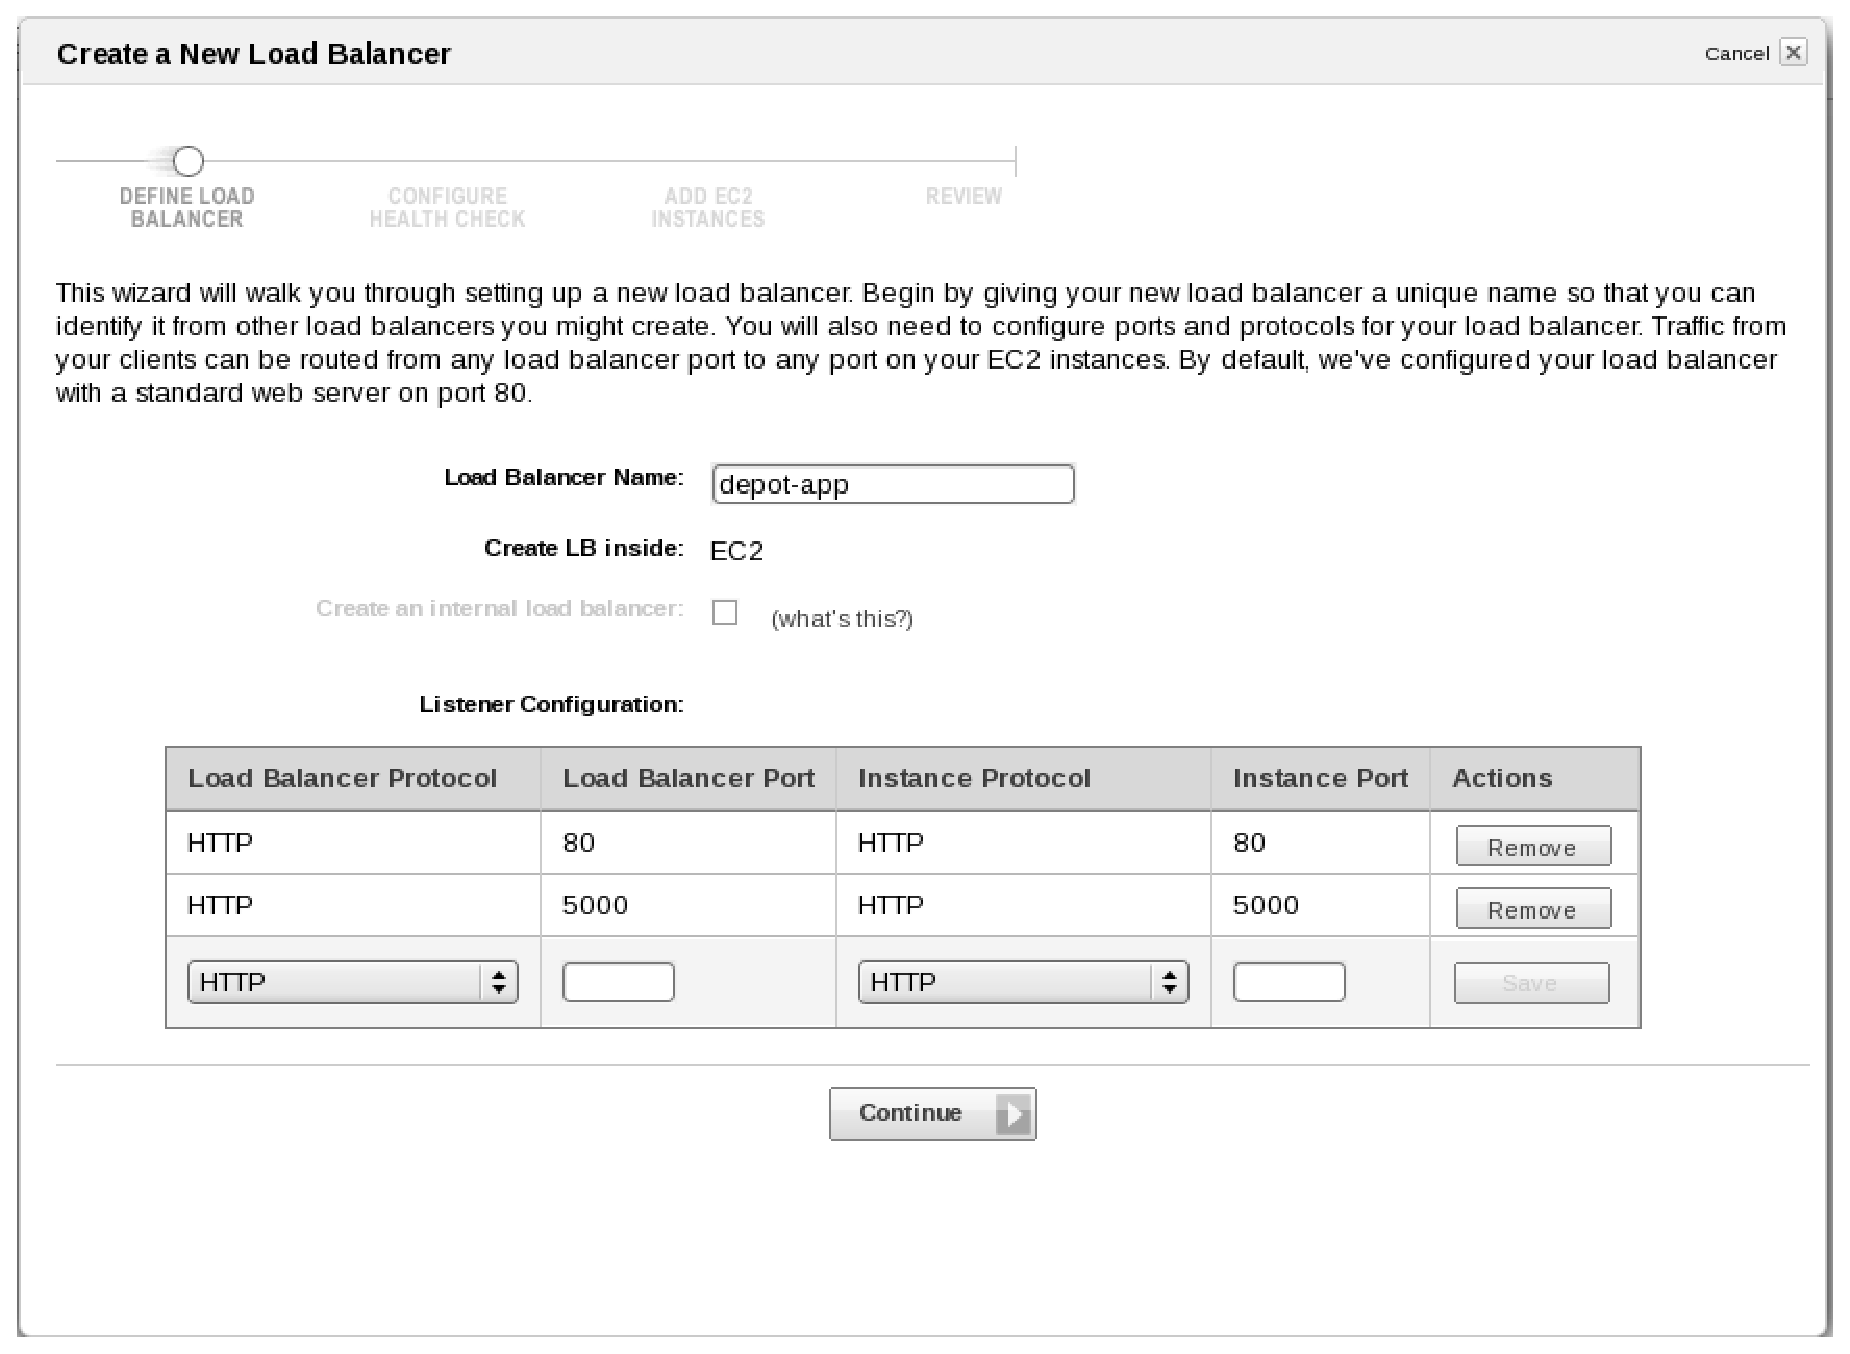
\includegraphics[scale=0.2]{createaelb0.eps}
\end{center}
\item Configure Health Check
\begin{center}

\includegraphics[scale=0.2]{createaelb.eps}
\end{center}	
\item Add \acrshort{ec2} instances
\item Review
\end{enumerate}

\end{frame}
%%%%%%%%%%%%%%%%%%%%%%%%%%%%%%%%%%%%%%%%%%%%%%%%%%%%%%%%%%%%%%%%%%%%%%%%%%%%%%
%%%%%%%%%%%%%%%%%%%%%%%%%%%%%%%%%%%%%%%%%%%%%%%%%%%%%%%%%%%%%%%%%%%%%%%%%%%%%%
\begin{frame}[fragile, allowframebreaks]
\frametitle{Testing a ELB}
\
\begin{enumerate}	
\item Curl the fully qualified domain name of \acrshort{elb} in order to test \acrshort{elb} the address info
\lstset{language=shell}
\begin{lstlisting}[escapechar=!]
$ curl http://depot-app-1557778043.us-east-1.elb.amazonaws.com:5000 2>/dev/null | grep 'Addrinfo:' | gawk '{print $4}'
!\outputcommand{10.192.182.72\&gt;,}!
$ curl http://depot-app-1557778043.us-east-1.elb.amazonaws.com:5000 2>/dev/null | grep 'Addrinfo:' | gawk '{print $4}'
!\outputcommand{10.210.202.71\&gt;,}!
\end{lstlisting}
\end{enumerate}

\end{frame}
%%%%%%%%%%%%%%%%%%%%%%%%%%%%%%%%%%%%%%%%%%%%%%%%%%%%%%%%%%%%%%%%%%%%%%%%%%%%%%
%%%%%%%%%%%%%%%%%%%%%%%%%%%%%%%%%%%%%%%%%%%%%%%%%%%%%%%%%%%%%%%%%%%%%%%%%%%%%%
\section{AutoScaling}
%%%%%%%%%%%%%%%%%%%%%%%%%%%%%%%%%%%%%%%%%%%%%%%%%%%%%%%%%%%%%%%%%%%%%%%%%%%%%%
%%%%%%%%%%%%%%%%%%%%%%%%%%%%%%%%%%%%%%%%%%%%%%%%%%%%%%%%%%%%%%%%%%%%%%%%%%%%%%%%%%%%%%%%%%%%%%%%%%%%%%%%%%%%%%%%%%%%%%%%%%%%%%%%%%%%%%%%%%
\begin{frame}[fragile, allowframebreaks]
\frametitle{Auto Scaling}
\begin{itemize}
 \item Auto Scaling is a web service that enables you to automatically launch or terminate \acrshort{ec2} instances based on user-defined policies, health status checks, and schedules
 \item Scaling is the ability to increase or decrease the compute capacity of your application by either changing the number of servers (horizontal scaling) or changing the size of the servers (vertical scaling)
\item The decision when to scale vertically and when to scale horizontally depends on factors such as your use case, cost, performance, and infrastructure
\item Auto Scaling allows you to scale your compute resources dynamically and predictably:
\begin{itemize}
 \item Dynamically based on conditions specified by you (for example, increasing CPU utilization of your \acrshort{ec2} instance)
 \item Predictably according to a schedule defined by you (for example, every Friday at 13:00:00)
\end{itemize}

\end{itemize}

\begin{center}
 \item 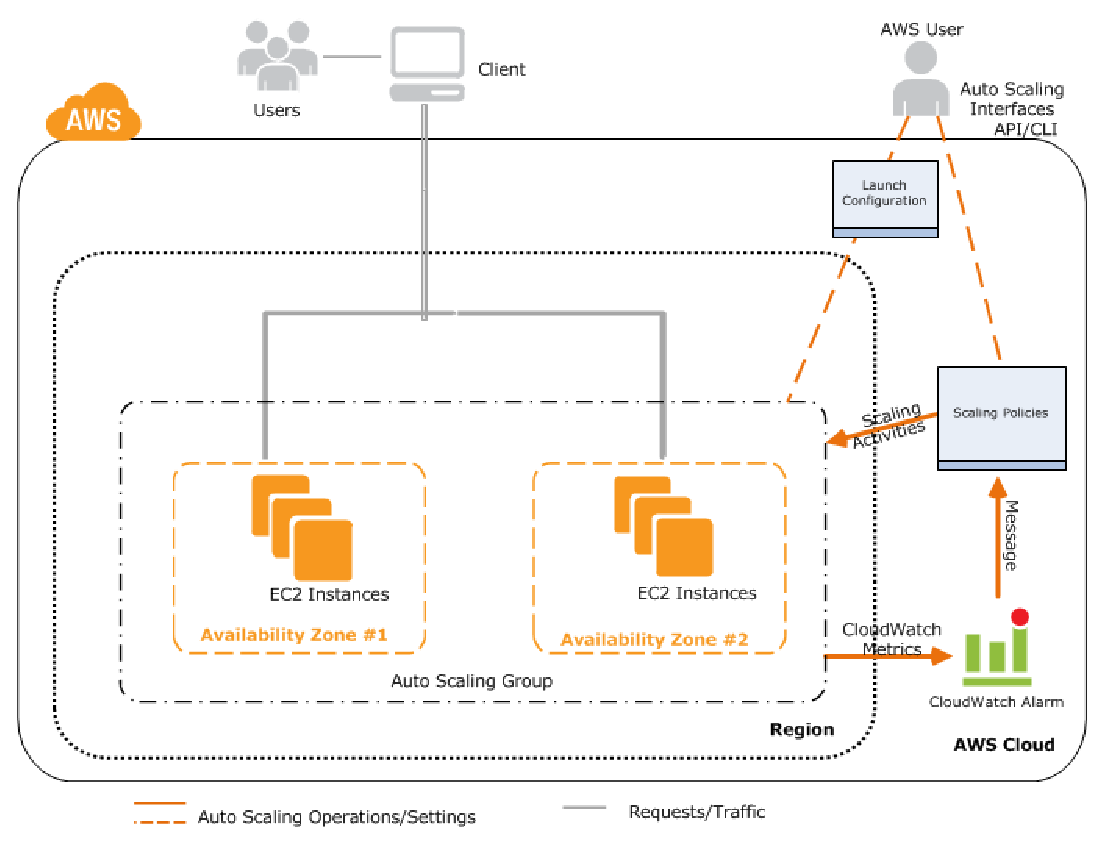
\includegraphics[scale=0.4]{AS-WorkFlow.eps}
\end{center}

\end{frame}

%%%%%%%%%%%%%%%%%%%%%%%%%%%%%%%%%%%%%%%%%%%%%%%%%%%%%%%%%%%%%%%%%%%%%%%%%%%%%%%%%%%%%%%%%%%%%%%%%%%%%%%%%%%%%%%%%%%%%%%%%%%%%%%%%%%%%%%%%%
\begin{frame}[fragile, allowframebreaks]
\frametitle{Launch Configuration and Auto Scaling Group}
\begin{enumerate}
\item Created a launch configuration by providing all the information required to launch EC2 instances
\begin{enumerate}
\item Choose \acrshort{ami} among ``My AMIs'' or ``AWS Marketplace'' or ``Community AMIs''
\item Choose Instance Type among  ``micro'', ``small'', ``medium'', \dots
\item Configure details: ``Name'', ``Purchasing option (Request Spot Instances)'', ``IAM Role'' and  ``Monitoring (Enable CloudWatch detailed monitoring)''
\item Add Storage
\item Configure Security Group
\item Review
\end{enumerate}
\item Created an Auto Scaling group by defining maximum, minimum, and (optionally), the desired capacity for the EC2 instances
\begin{enumerate}
\item Configure Auto Scaling group details: ``Launch Configuration'', ``Group name'',  ``Group size Start with \texttt{n} instances'', ``Network'', ``Availability Zone(s)''
\item Configure scaling policies ``Keep this group at its initial size'' or ``Use scaling policies to adjust the capacity of this group''
\item Configure Notifications (Configure your Auto Scaling group to send notifications to a specified endpoint, such as an email address, whenever a specified event takes place, including: successful launch of an instance, failed instance launch, instance termination, and failed instance termination)
\item Review
\end{enumerate}
\item Created an Amazon CloudWatch alarm and defined which metrics to monitor
\item Created two scaling policies, one for scaling out and another for scaling in, and associated the policies with the alarm
\item Associated the scaling policies with the Auto Scaling group
\end{enumerate}

\end{frame}
%%%%%%%%%%%%%%%%%%%%%%%%%%%%%%%%%%%%%%%%%%%%%%%%%%%%%%%%%%%%%%%%%%%%%%%%%%%%%%%%%%%%%%%%%%%%%%%%%%%%%%%%%%%%%%%%%%%%%%%%%%%%%%%%%%%%%%%%%%
%%%%%%%%%%%%%%%%%%%%%%%%%%%%%%%%%%%%%%%%%%%%%%%%%%%%%%%%%%%%%%%%%%%%%%%%%%%%%%%%%%%%%%%%%%%%%%%%%%%%%%%%%%%%%%%%%%%%%%%%%%%%%%%%%%%%%%%%%%
\begin{frame}[fragile, allowframebreaks]
\frametitle{Alarm and Policy}
\begin{itemize}
\item An Auto Scaling group uses a combination of \emph{policies} and \emph{alarms} to determine when the specified conditions for launching and terminating instances are met
\item An \emph{alarm} is an object that watches over a single metric (for example, the average CPU utilization of your EC2 instances in an Auto Scaling group) over a time period that you specify. When the value of the metric breaches the thresholds that you define, over a number of time periods that you specify, the alarm performs one or more actions. An action can be sending messages to Auto Scaling
\item A \emph{policy} is a set of instructions for Auto Scaling that tells the service how to respond to alarm messages
\item Along with creating a launch configuration and Auto Scaling group, you need to create the alarms and the scaling policies and associate them with your Auto Scaling group. When the alarm sends the message, Auto Scaling executes the associated policy on your Auto Scaling group to scale the group in (that is, to terminate instances) or scale the group out (that is, to launch instances).
\end{itemize}

\end{frame}
%%%%%%%%%%%%%%%%%%%%%%%%%%%%%%%%%%%%%%%%%%%%%%%%%%%%%%%%%%%%%%%%%%%%%%%%%%%%%%%%%%%%%%%%%%%%%%%%%%%%%%%%%%%%%%%%%%%%%%%%%%%%%%%%%%%%%%%%%%

\end{document}

